% Created by tikzDevice version 0.12 on 2018-09-20 18:03:19
% !TEX encoding = UTF-8 Unicode
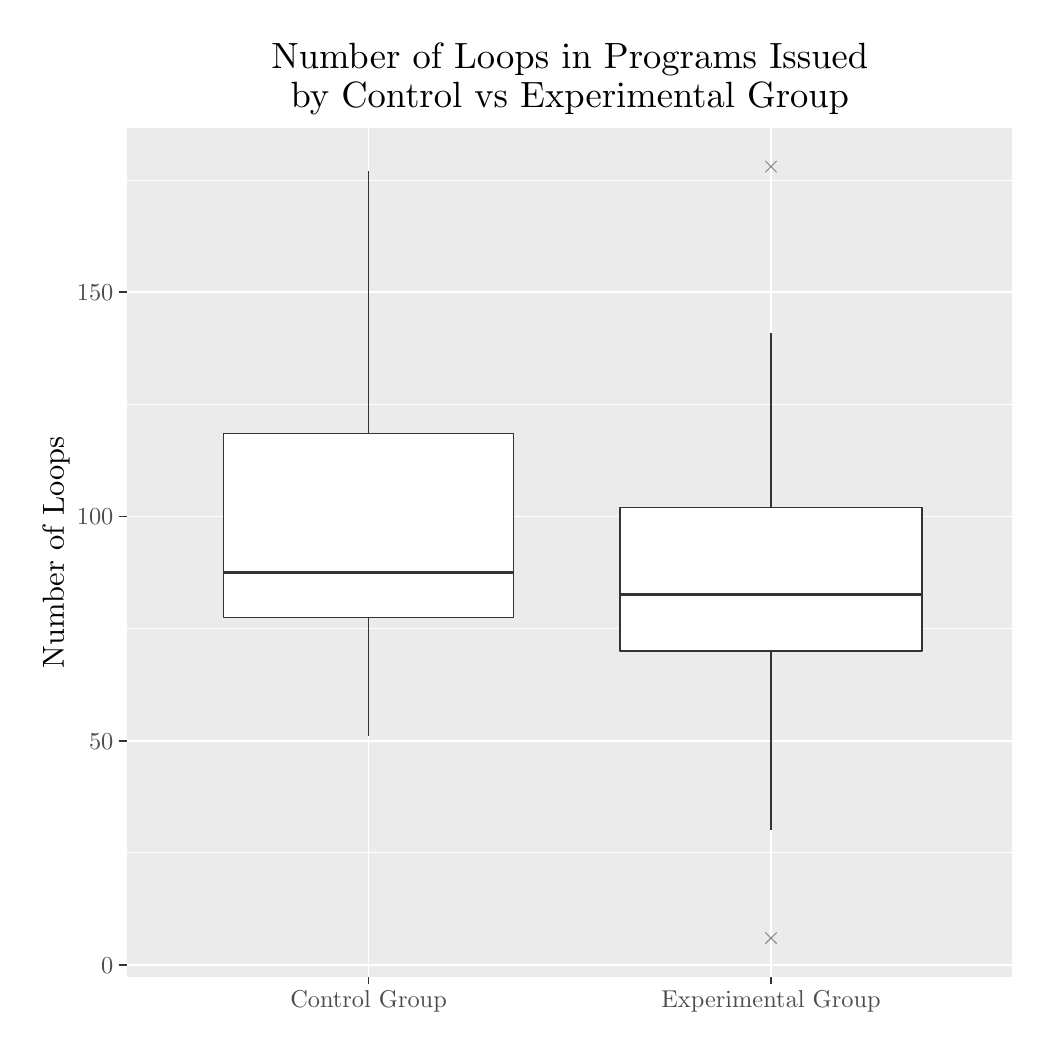
\begin{tikzpicture}[x=1pt,y=1pt]
\definecolor{fillColor}{RGB}{255,255,255}
\path[use as bounding box,fill=fillColor,fill opacity=0.00] (0,0) rectangle (361.35,361.35);
\begin{scope}
\path[clip] (  0.00,  0.00) rectangle (361.35,361.35);
\definecolor{drawColor}{RGB}{255,255,255}
\definecolor{fillColor}{RGB}{255,255,255}

\path[draw=drawColor,line width= 0.6pt,line join=round,line cap=round,fill=fillColor] (  0.00,  0.00) rectangle (361.35,361.35);
\end{scope}
\begin{scope}
\path[clip] ( 35.92, 18.45) rectangle (355.85,325.06);
\definecolor{fillColor}{gray}{0.92}

\path[fill=fillColor] ( 35.92, 18.45) rectangle (355.85,325.06);
\definecolor{drawColor}{RGB}{255,255,255}

\path[draw=drawColor,line width= 0.3pt,line join=round] ( 35.92, 63.18) --
	(355.85, 63.18);

\path[draw=drawColor,line width= 0.3pt,line join=round] ( 35.92,144.21) --
	(355.85,144.21);

\path[draw=drawColor,line width= 0.3pt,line join=round] ( 35.92,225.23) --
	(355.85,225.23);

\path[draw=drawColor,line width= 0.3pt,line join=round] ( 35.92,306.26) --
	(355.85,306.26);

\path[draw=drawColor,line width= 0.6pt,line join=round] ( 35.92, 22.67) --
	(355.85, 22.67);

\path[draw=drawColor,line width= 0.6pt,line join=round] ( 35.92,103.69) --
	(355.85,103.69);

\path[draw=drawColor,line width= 0.6pt,line join=round] ( 35.92,184.72) --
	(355.85,184.72);

\path[draw=drawColor,line width= 0.6pt,line join=round] ( 35.92,265.75) --
	(355.85,265.75);

\path[draw=drawColor,line width= 0.6pt,line join=round] (123.17, 18.45) --
	(123.17,325.06);

\path[draw=drawColor,line width= 0.6pt,line join=round] (268.60, 18.45) --
	(268.60,325.06);
\definecolor{drawColor}{RGB}{51,51,51}

\path[draw=drawColor,draw opacity=0.50,line width= 0.4pt,line join=round,line cap=round] (266.63, 30.43) -- (270.56, 34.35);

\path[draw=drawColor,draw opacity=0.50,line width= 0.4pt,line join=round,line cap=round] (266.63, 34.35) -- (270.56, 30.43);

\path[draw=drawColor,draw opacity=0.50,line width= 0.4pt,line join=round,line cap=round] (266.63,309.16) -- (270.56,313.08);

\path[draw=drawColor,draw opacity=0.50,line width= 0.4pt,line join=round,line cap=round] (266.63,313.08) -- (270.56,309.16);
\definecolor{drawColor}{gray}{0.20}

\path[draw=drawColor,line width= 0.6pt,line join=round] (268.60,187.96) -- (268.60,251.16);

\path[draw=drawColor,line width= 0.6pt,line join=round] (268.60,136.11) -- (268.60, 71.28);
\definecolor{fillColor}{RGB}{255,255,255}

\path[draw=drawColor,line width= 0.6pt,line join=round,line cap=round,fill=fillColor] (214.06,187.96) --
	(214.06,136.11) --
	(323.13,136.11) --
	(323.13,187.96) --
	(214.06,187.96) --
	cycle;

\path[draw=drawColor,line width= 1.1pt,line join=round] (214.06,156.36) -- (323.13,156.36);

\path[draw=drawColor,line width= 0.6pt,line join=round] (123.17,214.70) -- (123.17,309.50);

\path[draw=drawColor,line width= 0.6pt,line join=round] (123.17,148.26) -- (123.17,105.32);

\path[draw=drawColor,line width= 0.6pt,line join=round,line cap=round,fill=fillColor] ( 70.78,214.70) --
	( 70.78,148.26) --
	(175.57,148.26) --
	(175.57,214.70) --
	( 70.78,214.70) --
	cycle;

\path[draw=drawColor,line width= 1.1pt,line join=round] ( 70.78,164.46) -- (175.57,164.46);
\end{scope}
\begin{scope}
\path[clip] (  0.00,  0.00) rectangle (361.35,361.35);
\definecolor{drawColor}{gray}{0.30}

\node[text=drawColor,anchor=base east,inner sep=0pt, outer sep=0pt, scale=  0.88] at ( 30.97, 19.64) {0};

\node[text=drawColor,anchor=base east,inner sep=0pt, outer sep=0pt, scale=  0.88] at ( 30.97,100.66) {50};

\node[text=drawColor,anchor=base east,inner sep=0pt, outer sep=0pt, scale=  0.88] at ( 30.97,181.69) {100};

\node[text=drawColor,anchor=base east,inner sep=0pt, outer sep=0pt, scale=  0.88] at ( 30.97,262.72) {150};
\end{scope}
\begin{scope}
\path[clip] (  0.00,  0.00) rectangle (361.35,361.35);
\definecolor{drawColor}{gray}{0.20}

\path[draw=drawColor,line width= 0.6pt,line join=round] ( 33.17, 22.67) --
	( 35.92, 22.67);

\path[draw=drawColor,line width= 0.6pt,line join=round] ( 33.17,103.69) --
	( 35.92,103.69);

\path[draw=drawColor,line width= 0.6pt,line join=round] ( 33.17,184.72) --
	( 35.92,184.72);

\path[draw=drawColor,line width= 0.6pt,line join=round] ( 33.17,265.75) --
	( 35.92,265.75);
\end{scope}
\begin{scope}
\path[clip] (  0.00,  0.00) rectangle (361.35,361.35);
\definecolor{drawColor}{gray}{0.20}

\path[draw=drawColor,line width= 0.6pt,line join=round] (123.17, 15.70) --
	(123.17, 18.45);

\path[draw=drawColor,line width= 0.6pt,line join=round] (268.60, 15.70) --
	(268.60, 18.45);
\end{scope}
\begin{scope}
\path[clip] (  0.00,  0.00) rectangle (361.35,361.35);
\definecolor{drawColor}{gray}{0.30}

\node[text=drawColor,anchor=base,inner sep=0pt, outer sep=0pt, scale=  0.88] at (123.17,  7.44) {Control Group};

\node[text=drawColor,anchor=base,inner sep=0pt, outer sep=0pt, scale=  0.88] at (268.60,  7.44) {Experimental Group};
\end{scope}
\begin{scope}
\path[clip] (  0.00,  0.00) rectangle (361.35,361.35);
\definecolor{drawColor}{RGB}{0,0,0}

\node[text=drawColor,rotate= 90.00,anchor=base,inner sep=0pt, outer sep=0pt, scale=  1.10] at ( 13.08,171.76) {Number of Loops};
\end{scope}
\begin{scope}
\path[clip] (  0.00,  0.00) rectangle (361.35,361.35);
\definecolor{drawColor}{RGB}{0,0,0}

\node[text=drawColor,anchor=base,inner sep=0pt, outer sep=0pt, scale=  1.32] at (195.88,346.76) {Number of Loops in Programs Issued};

\node[text=drawColor,anchor=base,inner sep=0pt, outer sep=0pt, scale=  1.32] at (195.88,332.50) {by Control vs Experimental Group};
\end{scope}
\end{tikzpicture}
